\documentclass{article}

\usepackage[a4paper, margin=0.95cm, landscape]{geometry}
% \usepackage[utf8]{inputenc}
\usepackage[scaled]{helvet}
\usepackage[rgb]{xcolor}
\usepackage[british]{babel}
\usepackage{pgfkeys}
\usepackage{xparse}
\usepackage{etoolbox}
\usepackage[fixed]{fontawesome5}
\usepackage{xstring}
\usepackage{pgfornament}
\usepackage{graphicx}
\usepackage{setspace}
\usepackage{enumitem}
\usepackage{amssymb}

\usepackage{tikz}
\usetikzlibrary{shadows.blur}
\usetikzlibrary{positioning,shapes.misc}
\usetikzlibrary{patterns}
\usetikzlibrary{math}
\usetikzlibrary{patterns.meta}
\usetikzlibrary{fit}
\pagenumbering{gobble}

\newcommand{\cardwidth}{41}
\newcommand{\cardheight}{63}

\pgfqkeys{/cardkeys}{
  fontsize/.store in=\textsize,
  type/.store in=\type,
  time/.store in=\time,
  cost/.store in=\cost,
  components/.store in=\components,
  cost/.store in=\cost,
  type/.store in=\type,
  time/.store in=\time,
  components/.store in=\components,
  ac/.store in=\ac,
  hp/.store in=\hp,
  speed/.store in=\speed,
  speedm/.store in=\speedm,
  prof/.store in=\prof,
  perc/.store in=\perc,
  str/.store in=\str,
  strb/.store in=\strb,
  dex/.store in=\dex,
  dexb/.store in=\dexb,
  con/.store in=\con,
  conb/.store in=\conb,
  int/.store in=\int,
  intb/.store in=\intb,
  wis/.store in=\wis,
  wisb/.store in=\wisb,
  cha/.store in=\cha,
  chab/.store in=\chab,
  fontsize=6,
  cost=,
  type=,
  time=,
  components=,
  ac=,
  hp=,
  speed=,
  speedm=,
  prof=,
  perc=,
  str=,
  strb=,
  dex=,
  dexb=,
  con=,
  conb=,
  int=,
  intb=,
  wis=,
  wisb=,
  cha=,
  chab=
}

\tikzstyle{tag}=[
        fill=black, 
        draw=black, 
        inner sep=0.75mm, 
        anchor=east,
        font=\sffamily\fontsize{4}{4}\selectfont\color{white},
        rounded corners=0.4mm
]

\tikzstyle{greentag}=[tag, fill=green, draw=green!70!black]
\tikzstyle{redtag}=[tag, fill=red, draw=red!70!black]
\tikzstyle{bluetag}=[tag, fill=blue, draw=blue!70!black]
\tikzstyle{yellowtag}=[tag, fill=yellow, draw=yellow!70!black]
\tikzstyle{orangetag}=[tag, fill=orange, draw=orange!70!black]
\tikzstyle{tealtag}=[tag, fill=teal, draw=teal!70!black]
\tikzstyle{purpletag}=[tag, fill=purple, draw=purple!70!black]

\tikzstyle{title}=[
    fill=white, 
    draw=black, 
    minimum width=37mm, 
    inner sep=1mm, 
    fill opacity=.5,
    text opacity=1, 
    font=\sffamily\fontsize{7}{7}\selectfont,
    rounded corners=0.4mm
]
        
\tikzstyle{floatingbox}=[
    fill=parchment, 
    draw=black, 
    minimum width=37mm, 
    inner sep=2mm, 
    fill opacity=.6,
    text opacity=1, 
    draw opacity=1,
    rounded corners=0.4mm
]

\tikzstyle{footnotes}=[
    inner sep=2mm, 
    text width=20mm, 
    font=\sffamily\fontsize{4}{4.5}\selectfont
]

% ===========================
% Remove espaçamento vertical
% ===========================
\newcommand{\removespace}{\vspace{-0.35mm}}

% ===========================
% CARDS
% ===========================
\newcommand{\card}[5][]{%
    \begingroup\pgfqkeys{/cardkeys}{#1}%
    \begin{tikzpicture}[x=1mm, y=1mm]
    
        \tikzmath{\fs = \textsize + 0.5;}
        
        % Parchment paper
        \draw[fill=parchment] (0,0) rectangle (\cardwidth,\cardheight);
    
        % Imagem
        \node[anchor=north west, inner sep=0,outer sep=0] (image) at (0, 63) {\includegraphics[width=41mm]{#2}};
    
        % Título
        \node[title, anchor=north west](title) at (2,61) {\textbf{#3}};
    
        % Texto
        \node[fill=parchment, inner sep=2mm, outer sep=0, font=\sffamily\fontsize{\textsize}{\fs}\selectfont, text width=37mm, anchor=north west, align=justify] (text) at (0, 42) {#4};
    
        % Separador
        \draw [line width = 0.5mm] ([yshift=0.25mm] text.north west) -- ([yshift=0.25mm] text.north east);
    
        \coordinate (tagpos) at (39,3);
    
        % Type
        \ifdefstring{\type}{}{}{\node[tag](type) at (39, 42) {\MakeUppercase{\textbf{\type}}};}
    
        % Time
        \ifdefstring{\time}{bonus}{\node[greentag](time) at (tagpos) {\MakeUppercase{\textbf{\time}}};\coordinate (tagpos) at ([xshift=-1mm] time.west);}{
            \ifdefstring{\time}{action}{\node[bluetag](time) at (tagpos) {\MakeUppercase{\textbf{\time}}};\coordinate (tagpos) at ([xshift=-1mm] time.west);}{
                \ifdefstring{\time}{reaction}{\node[redtag](time) at (tagpos) {\MakeUppercase{\textbf{\time}}};\coordinate (tagpos) at ([xshift=-1mm] time.west);}{
                    \ifdefstring{\time}{}{}{
                        \node[redtag](time) at (tagpos) {\MakeUppercase{\textbf{\time}}};
                        \coordinate (tagpos) at ([xshift=-1mm] time.west);
        }}}}
    
        % Cost
        \ifdefstring{\cost}{}{}{
            \ifdefstring{\cost}{at-will}{
                \node[tag, opacity=0.1, text opacity=0.7](cost) at (tagpos) {\color{black}\MakeUppercase{\textbf{\cost}}};
            }{
                \node[tag](cost) at (tagpos) {\MakeUppercase{\textbf{\cost}}};
            }
            \coordinate (tagpos) at ([xshift=-1mm] cost.west);
        }
        
        % Components
        \ifdefstring{\components}{}{}{
            \node[tag, opacity=0.1, text opacity=0.7](componentes) at (tagpos) {%
                \color{black}%
                \IfSubStr{\components}{V}{\faIcon[solid]{comment}}{}%
                \IfSubStr{\components}{S}{\faIcon[solid]{hand-paper}}{}%
                \IfSubStr{\components}{M}{\faIcon[solid]{magic}}{}%
            };
            \coordinate (tagpos) at ([xshift=-1mm] componentes.west);
        }
        
    
        % Footnotes
        \node[footnotes, anchor=south west] (text) at (0, 0) {#5};
    
        % Borda
        \draw[line width = 0.5mm, black] (0,0) rectangle (\cardwidth,\cardheight);
    
    \end{tikzpicture}\endgroup\allowbreak }


% ===========================
% TOKEN
% ===========================
\newcommand{\token}[4][]{%
    \begingroup\pgfqkeys{/cardkeys}{#1}%
    \begin{tikzpicture}[x=1mm, y=1mm]
    
        \tikzmath{\fs = \textsize + 0.5;}
    
        % Imagem (trim: left, bottom, right, top
        \node[anchor=north west, inner sep=0, outer sep=0] (image) at (0, 63) {\includegraphics[width=41mm]{#2}};
    
        % Título
        \node[title, anchor=north west](title) at (2,61) {\textbf{#3}};
    
        % Texto
        \node[floatingbox, font=\sffamily\fontsize{\textsize}{\fs}\selectfont, text width=33mm, anchor=south, align=justify] (text) at (20.5, 2) {#4};
    
        % Type
        \ifdefstring{\type}{}{}{\node[tag](type) at ([xshift=-2mm] text.north east) {\MakeUppercase{\textbf{\type}}};}

        % Borda
        \draw[line width = 0.5mm, black] (0,0) rectangle (\cardwidth,\cardheight);
    
    \end{tikzpicture}\endgroup\allowbreak}

% ===========================
% EMPTY
% ===========================
\newcommand{\emptycard}{%
    
\begin{tikzpicture}[x=1mm, y=1mm]
        % Borda
        \draw[line width = 0.5mm, black] (0,0) rectangle (\cardwidth,\cardheight);
    \end{tikzpicture}}

% ===========================
% IMAGE ONLY
% ===========================
\newcommand{\imagecard}[1]{%
    \begin{tikzpicture}[x=1mm, y=1mm]
    
        % Imagem (trim: left, bottom, right, top
        \node[anchor=north west, inner sep=0,outer sep=0] (back) at (0, 63) {\includegraphics[width=41mm]{#1}};

        % Borda
        \draw[line width = 0.5mm, black] (0,0) rectangle (\cardwidth,\cardheight);
    
    \end{tikzpicture}\allowbreak}
% ===========================
% BACK CARDS
% ===========================
\newcommand{\backcard}[3][]{%
    \begingroup\pgfqkeys{/cardkeys}{#1}%
    \begin{tikzpicture}[x=1mm, y=1mm]
    
        % Imagem (trim: left, bottom, right, top
        \begin{scope}[blend group=color];
            \node[anchor=north west, inner sep=0,outer sep=0] (back) at (0, 63) {
\includegraphics[width=41mm]{images/back}};
            \fill[#2!50!black] (back.south west) rectangle (back.north east);
        \end{scope};
    
        
        \node[font=\sffamily\fontsize{8}{8}\selectfont, line width=0.3mm, rounded corners=0.8mm, draw=black, fill=black, text opacity=1, fill opacity=0.8, anchor=center, outer sep=0, inner sep=2mm] (center1) at (20.8, 7)  {\color{white}\MakeUppercase{\textbf{#3}}};
    
        % Borda
        \draw[line width = 0.5mm, black] (0,0) rectangle (\cardwidth,\cardheight);
    
    \end{tikzpicture}\endgroup\allowbreak}

% ===========================
% PET
% ===========================
\newcommand{\pet}[5][]{%
    \begingroup\pgfqkeys{/cardkeys}{#1}%
    \begin{tikzpicture}[x=1mm, y=1mm]
    
        \tikzmath{\fs = \textsize + 0.5;}
        
        % Parchment paper
        \draw[fill=parchment] (0,0) rectangle (\cardwidth,\cardheight);
    
        % Imagem
        \node[anchor=north west, inner sep=0,outer sep=0] (back) at (0, 63) {\includegraphics[width=41mm]{#2}};    

        % Título
        \node[title, anchor=north west](title) at (2,61) {\textbf{#3}};
    
        % % Texto
        % \node[fill=parchment, inner sep=2mm, outer sep=0, font=\sffamily\fontsize{\textsize}{\fs}\selectfont, text width=37mm, anchor=north west, align=justify] (text) at (0, 42) {#4};
        
        % Stats
        \centerbox[anchor=north west, minimum height=6mm, minimum width=6mm]{1.5, 55}{AC}{\ac}
        \centerbox[anchor=north west, minimum height=6mm, minimum width=6mm]{9.5, 55}{HP}{\hp}
        \centerbox[anchor=north west, minimum height=6mm, minimum width=6mm]{17.5, 55}{SPEED}{\speed}
        \centerbox[anchor=north west, minimum height=6mm, minimum width=6mm]{25.5, 55}{PROF}{\prof}
        \centerbox[anchor=north west, minimum height=6mm, minimum width=6mm]{33.5, 55}{PERC}{\perc} 
        
        % Atributos
        \node[fill=parchment, opacity=0.7, text opacity=1, draw opacity=1, inner sep=0mm, anchor=north west, font=\sffamily\fontsize{8}{8.5}, draw=black, rounded corners=0.4mm, fit={(1.5,28) (15.5,12)}] (ATTRS) {};
    
        \node[tag, anchor=east] at ([xshift=-0.5mm] ATTRS.north east) {ATTRS};
        
        \node[anchor=west, align=left, text width=3mm, font=\sffamily\fontsize{5}{6}\selectfont] (att) at (ATTRS.west) {%
        \textbf{STR}\\
        \textbf{DEX}\\
        \textbf{CON}\\
        \textbf{INT}\\
        \textbf{WIS}\\
        \textbf{CHA}
        };
        \node[anchor=west, align=right, minimum width=4mm, font=\sffamily\fontsize{5}{6}\selectfont] (att2) at (att.east) {%
        \str\\
        \dex\\
        \con\\
        \int\\
        \wis\\
        \cha
        };
        \node[anchor=west, align=center, font=\sffamily\fontsize{5}{6}\selectfont] (att3) at ([xshift=2.5mm] att.east) {%
        (\strb)\\
        (\dexb)\\
        (\conb)\\
        (\intb)\\
        (\wisb)\\
        (\chab)
        };
    

        % SKILLS
        \node[fill=parchment, opacity=0.7, text opacity=1, draw opacity=1, inner sep=0mm, anchor=north west, font=\sffamily\fontsize{8}{8.5}, draw=black, rounded corners=0.4mm, fit={(1.5, 10) (15.5, 2)}] (SKILLS) {};
    
        \node[tag, anchor=east] at ([xshift=-0.5mm] SKILLS.north east) {SKILLS};
        
        \node[anchor=west, align=left, text width=14mm, font=\sffamily\fontsize{4}{4.5}\selectfont] (sk) at (SKILLS.west) {%
        #4
        };

        % ABILITIES
        \node[fill=parchment, opacity=0.7, text opacity=1, draw opacity=1, inner sep=0mm, anchor=north west, font=\sffamily\fontsize{8}{8.5}, draw=black, rounded corners=0.4mm, fit={(17.5, 28) (39.5, 2)}] (ABS) {};
    
        \node[tag, anchor=east] at ([xshift=-0.5mm] ABS.north east) {ABILITIES AND ATTACKS};
        
        \node[anchor=west, align=left, text width=18mm, font=\sffamily\fontsize{4.5}{4.5}\selectfont] (ab) at (ABS.west) {%
        #5
        };
        
        % Borda
        \draw[line width = 0.5mm, black] (0,0) rectangle (\cardwidth,\cardheight);
    
    \end{tikzpicture}\endgroup\allowbreak }
% ============================    
% CHARACTER SHEET
% ============================    
\tikzstyle{squarebox}=[
    inner sep=1mm, 
    fill=parchment, 
    opacity=0.7, 
    text opacity=1, 
    draw opacity=1,
    draw=black, 
    %  width=6mm, 
    inner sep=0mm,
    minimum height=6mm, 
    minimum width=8mm, 
    rounded corners=0.5mm,
    font=\sffamily\fontsize{7}{7.5}
]

\tikzstyle{attribute}=[
    squarebox,
    text width=5mm,
    inner sep=2mm,
    font=\sffamily
]

\tikzstyle{subattribute}=[
    tag, 
    fill=parchment,
    inner sep=0.5mm,
    font=\sffamily\fontsize{5}{5}\selectfont%\color{white}
]

\newcommand{\leftbox}[5]{%
    \node[attribute, anchor=west] (#2) at (#1) {\textbf{#3}};
    \node[tag, anchor=west, xshift=0.5mm] at (#2.north west) {\textbf{#2}};
    \node[subattribute, anchor=north east, xshift=0.5mm, yshift=-0.5mm] at (#2.north east) {\textbf{#4}};
    \node[subattribute, anchor=south east, xshift=0.5mm, yshift=0.5mm] at (#2.south east) {\textbf{#5}};
}

\newcommand{\rightbox}[5]{%
    \node[attribute, anchor=east, align=right] (#2) at (#1) {\textbf{#3}};
    \node[tag, anchor=east, xshift=-0.5mm] at (#2.north east) {\textbf{#2}};
    \node[subattribute, anchor=north west, xshift=-0.5mm, yshift=-0.5mm] at (#2.north west) {\textbf{#4}};
    \node[subattribute, anchor=south west, xshift=-0.5mm, yshift=0.5mm] at (#2.south west) {\textbf{#5}};
}

\newcommand{\centerbox}[4][]{%
    \node[squarebox, anchor=center, #1] (#3) at (#2) {\textbf{#4}};
    \node[tag, anchor=center] at (#3.north) {\textbf{#3}};
}

\newcommand{\centerboxsubs}[5][]{%
    \node[squarebox, anchor=center, #1] (#3) at (#2) {\textbf{#4}};
    \node[tag, anchor=center] at (#3.north) {\textbf{#3}};
    % \node[subattribute, anchor=south west] at ([xshift=-0.5mm, yshift=-0.5mm]#3.south west) {\textbf{#5}};
    \node[subattribute, anchor=south east] at ([xshift=0.5mm, yshift=-0.7mm] #3.south east) {\textbf{#5}};
}


\begin{document}

\begin{tikzpicture}[x=1mm, y=1mm]

    \tikzmath{\fs = \textsize + 0.5;}
    
    % Parchment paper
    \draw[fill=parchment] (0,0) rectangle (63,88);

    % Imagem
    \node[anchor=north west, inner sep=0,outer sep=0] (image) at (0, 88) {
\includegraphics[width=63mm, height=88mm]{images/big-sig-saranova.png}};
    
    % Título
    \node[title, anchor=north west, minimum width=59mm](title) at (2,86) {\textbf{Sig Saranova}, Human Warlock 8, Hermit Neutral Good};

    % Atributos
    \leftbox{2,76.5}{STR}{+0}{10}{+0}
    \leftbox{2,68}{DEX}{+3}{16}{+3}
    \leftbox{2,59.5}{CON}{+2}{14}{+2}

    \rightbox{61,76.5}{INT}{+2}{14}{+2}
    \rightbox{61,68}{WIS}{+0}{10}{+3}
    \rightbox{61,59.5}{CHA}{+4}{19}{+7}
    
    % \node[xshift=0.1mm, yshift=-0.1mm] (div1) at (31.5, 55) {\color{white}\pgfornament[width=50mm]{86}};    
    % \node[opacity=1, xshift=0mm, yshift=-0.1mm] (div1) at (31.5, 55) {\color{white}\pgfornament[width=59mm]{86}};  
    % \node[opacity=1] (div1) at (31.5, 55) {\pgfornament[width=59mm]{86}};
    
    \centerbox[anchor=north west]{2, 52}{INIT}{+3}
    \centerbox[anchor=north west]{12, 52}{AC}{16}
    \centerbox[anchor=north west]{22, 52}{HP}{50}
    \centerbox[anchor=north west]{33, 52}{PROF}{+3}
    \centerbox[anchor=north west]{43, 52}{H DICE}{7d8}
    \centerboxsubs[anchor=north west]{53, 52}{SPEED}{9m}{30ft}

    \centerbox[anchor=north west]{22, 43}{SP ATT}{+8}
    \centerbox[anchor=north west]{32, 43}{SP SAVE}{16}
    \centerbox[anchor=north west]{43, 43}{SP SLOTS}{2}
    \centerbox[anchor=north west]{53, 43}{SP LEVEL}{4th}
    % \centerbox[anchor=north west]{53, 43}{}{}
    
    \node[fill=parchment, opacity=0.7, text opacity=1, draw opacity=1, inner sep=0mm, anchor=north west, font=\sffamily\fontsize{8}{8.5}, draw=black, rounded corners=0.4mm, fit={(2,43) (20,2)}] (SKILLS) {};
    
    \node[tag, anchor=east] at ([xshift=-0.5mm] SKILLS.north east) {SKILLS};

    \node[anchor=west, align=left, text width=3mm, font=\sffamily\fontsize{5}{6}\selectfont] (skvalues) at (SKILLS.west) {%
        +0\\ % Athletics\\
        +3\\ % Acrobatics\\
        +3\\ % Sleight of hand\\
        +3\\ % Stealth\\
        +5\\ % Arcana\\
        +2\\ % History\\
        +2\\ % Investigation\\
        +5\\ % Nature\\
        +5\\ % Religion\\
        +0\\ % Animal Handling\\
        +0\\ % Insight\\
        +3\\ % Medicine\\
        +0\\ % Perception\\
        +0\\ % Survival\\
        +4\\ % Deception\\
        +4\\ % Intimidation\\
        +4\\ % Performance\\
        +7\\ % Persuasion
        };

        \node[anchor=west, align=left, text width=13mm,font=\sffamily\fontsize{5}{6}\selectfont] (sknames) at ([xshift=3mm] SKILLS.west) {%
        Athletics\\
        {Acrobatics}\\
        Sleight of hand\\
        Stealth\\
        \textbf{Arcana}\\
        History\\
        Investigation\\
        \textbf{Nature}\\
        \textbf{Religion}\\
        Animal Handling\\
        {Insight}\\
        \textbf{Medicine}\\
        {Perception}\\
        Survival\\
        {Deception}\\
        Intimidation\\
        Performance\\
        \textbf{Persuasion}
        };

    \node[fill=parchment, opacity=0.7, text opacity=1, draw opacity=1, inner sep=0mm, anchor=north west, font=\sffamily\fontsize{8}{8.5}, draw=black, rounded corners=0.4mm, fit={(22,34) (61,8)}] (PROF) {};
    \node[tag, anchor=east] at ([xshift=-0.5mm] PROF.north east) {PROFICIENCIES AND ABILITIES};
    
    \node[anchor=west, align=left, text width=37mm, font=\sffamily\fontsize{4.4}{4.4}\selectfont] (feats) at (PROF.west) {%
        \textbf{Languages}: Common, celestial, dwarven.
        \\[0.7mm]
        \textbf{Armor and weapons}: Light armor, simple weapons.
        \\[0.7mm]
        \textbf{Pact Boon}: Pact of the Tome (Spare the Dying, guidance, message)
        \\[0.7mm]
        \textbf{Celestial}: Light and Sacred Flame cantrips, healing light, radiant soul (resistance vs radiant, char on spells of fire or radiant).
        \\[0.7mm]
        \textbf{Invocations}: Armor of shadows (mage armor), Agonizing blast (char on blast dmg), book of ancient secrets (find familiar, comprehend languages), skultor of flesh
        \\[0.7mm]
        \textbf{Feats}: Telekinetic feat (char +1, mage hand, Telekinetic)
        };


    \node[fill=parchment, opacity=0.7, text opacity=1, draw opacity=1, inner sep=0mm, anchor=north west, font=\sffamily\fontsize{8}{8.5}, draw=black, rounded corners=0.4mm, fit={(22,6) (61,2)}] (ATTACKS) {};
    
    \node[tag, anchor=east] at ([xshift=-0.5mm] ATTACKS.north east) {ATTACKS};

    \node[anchor=west, align=right, xshift=1mm, inner sep=0, font=\sffamily\fontsize{4.5}{6}\selectfont] (atts) at (ATTACKS.west) {%
        \textbf{Eldritch Blast (x2)}:
        };

    \node[anchor=west, align=left, text width=25mm, inner sep=0, xshift=0.5mm, font=\sffamily\fontsize{4.5}{6}\selectfont] (atts2) at (atts.east) {%
        +8, 1d10+4 force
        };



    % % Texto
    % \node[fill=parchment, inner sep=2mm, outer sep=0, font=\sffamily\fontsize{\textsize}{\fs}\selectfont, text width=37mm, anchor=north west, align=justify] (text) at (0, 55) {TEXTO1};

    % Borda
    \draw[line width = 0.5mm, black] (0,0) rectangle (63,88);

\end{tikzpicture}%
%
\begin{tikzpicture}[x=1mm, y=1mm]

    \tikzmath{\fs = \textsize + 0.5;}
    
    % Parchment paper
    \draw[fill=parchment] (0,0) rectangle (63,88);

    % Imagem
    \node[anchor=north west, inner sep=0,outer sep=0] (image) at (0, 88) {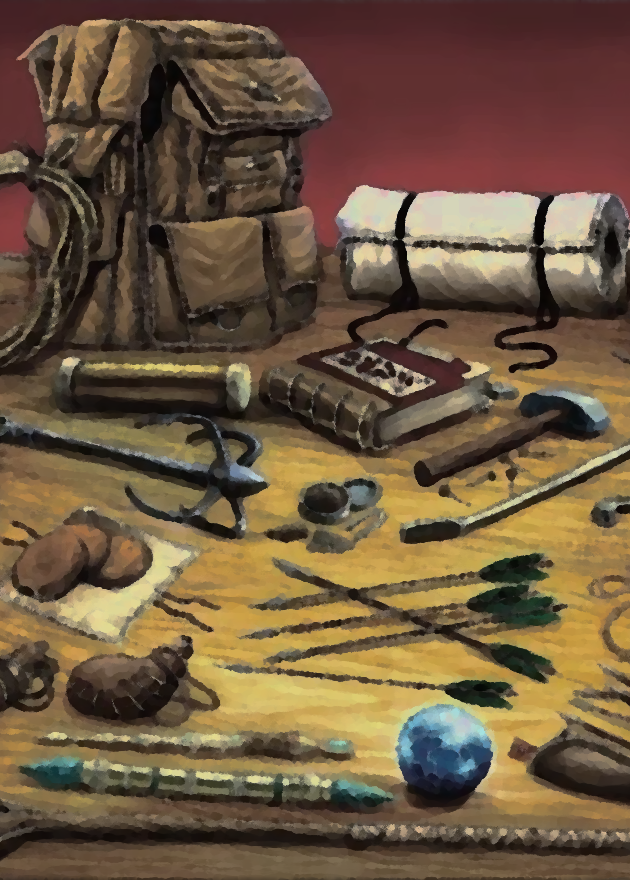
\includegraphics[width=63mm, height=88mm]{images/big-equipment.png}};
    
    % Título
    \node[title, anchor=north west, minimum width=59mm](title) at (2,86) {Equipments of \textbf{Sig Saranova}};

    \node[fill=parchment, opacity=0.7, text opacity=1, draw opacity=1, inner sep=0mm, anchor=north west, font=\sffamily\fontsize{8}{8.5}, draw=black, rounded corners=0.4mm, fit={(2,80) (51,2)}] (SKILLS) {};
    
    % \node[tag, anchor=east] at ([xshift=-0.5mm] SKILLS.north east) {SKILLS};
    
    \centerbox[anchor=north east]{61, 80}{COPP}{}
    \centerbox[anchor=north east]{61, 72}{SILV}{}
    \centerbox[anchor=north east, minimum height=3.8cm]{61, 64}{GOLD}{}
    \centerbox[anchor=north east]{61, 24}{PLAT}{}
    \centerbox[anchor=north east]{61, 16}{RATION}{}
    \centerbox[anchor=north east]{61, 8}{HEAL PT}{}

    \node[anchor=north west, align=left, text width=45mm, inner sep=2mm, font=\sffamily\fontsize{5}{6}\selectfont] (skvalues) at (SKILLS.north west) {
    \-- Backpack\\
    \-- Bedroll\\
    \-- Mess kit\\
    \-- Tinderbox\\
    \-- Waterskin\\
    \-- Rope (15m)\\
    \-- Books and scrolls\\
    \-- Blanket\\
    \-- Warm clothing\\
    \-- Herbalist kit\\
    \-- Barril de cerveja forte dos anões (1d4+1) $\square\square\square\square\square$\\
    \-- Cajado de vidro (CA+1, dez cargas mage armor (1) e shield (2))\\
    \-- Horses (x2)\\
    \-- Pearl of power\\
    \-- Boots of levitation\\
    \-- Rod of the pact keeper +1\\
    \-- Helm of Comprehending languages\\
    \-- Bússola de Localizar Objeto\\
    };

        

    % Borda
    \draw[line width = 0.5mm, black] (0,0) rectangle (63,88);

\end{tikzpicture}%

\newpage
%
\card[type=cantrip, time=action, cost=at-will, components=VS]{images/eldritch-blast}{Eldritch Blast}
    {A beam of crackling energy streaks toward a creature within range. Make a ranged spell Attack against the target. On a hit, the target takes 1d10 + 4 (Char by Agonizing Blast) force damage.
    \\[1mm]
    At Higher Levels. The spell creates more than one beam when you reach higher levels: two beams at 5th level, three beams at 11th level, and four beams at 17th level. You can direct the beams at the same target or at different ones. Make a separate attack roll for each beam.}
    {120 feet\\Instantaneous}%
\card[type=cantrip, time=action, cost=at-will, components=VS]{images/card-sacred-flame}{Sacred Flame}
    {Flame-like Radiance descends on a creature that you can see within range. The target must succeed on a Dexterity saving throw or take 2d8 + 4 (Char by Radiant Soul) radiant damage.
    \\[1mm]
    The target gains no benefit from cover for this saving throw.
    \\[1mm]
    At Higher Levels. The spell’s damage increases by 1d8 when you reach 5th level (2d8), 11th level (3d8), and 17th level (4d8).}
    {60 feet\\Instantaneous}%
\card[type=1st level spell, time=reaction, cost=spell, components=VS]{images/card-hellish-rebuke}{Hellish Rebuke}
    {You point your finger, and the creature that damaged you is momentarily surrounded by hellish flames. The creature must make a Dexterity saving throw.
    \\[1mm]
    It takes 5d10 + 4 (2d10 + 1d10 for each level over 1, +4 for char by radiant soul) fire damage on a failed save, or half as much damage on a successful one.}
    {60 feet\\Instantaneous}%
\card[type=1st level spell, time=action, cost=spell, components=VS]{images/card-mantra-of-healing}{Cure Wounds}
    {A creature you touch regains a number of Hit Points equal to 4d8 + 4 (1d8 + 1d8 for each spell level over 1st + your Spellcasting ability modifier).
    \\[1mm]
    This spell has no Effect on Undead or Constructs.}
    {Touch\\Instantaneous}%   
\card[type=2nd level spell, time=action, cost=spell, components=VSM]{images/card-invisibility}{Invisibility}
    {A creature you touch and two additional creatures (1 for each level over 2nd) becomes invisible until the spell ends. Anything the target is wearing or carrying is invisible as long as it is on the target’s person. The spell ends for a target that attacks or casts a spell.}
    {Touch\\Concentration, 1 hour}%
\card[type=3rd level spell, time=action, cost=spell, components=VS]{images/card-dispel-magic}{Dispel Magic}
    {Choose any creature, object, or magical effect within range. Any spell of 4th level or lower on the target ends. For each spell of 5th level or higher on the target, make an ability check using your spellcasting ability. The DC equals 10 + the spell’s level. On a successful check, the spell ends.
    \\[1mm]
    At Higher Levels. When you cast this spell using a spell slot of 4th level or higher, you automatically end the effects of a spell on the target if the spell’s level is equal to or less than the level of the spell slot you used.}
    {120 feet\\Instantaneous}%    
    
\removespace

\card[type=feat, time=bonus, cost=at-will]{images/card-telekinetic}{Telekinetic}
    {As a bonus action, you can try to telekinetically shove one creature you can see within 30 feet of you. When you do so, the target must succeed on a Strength saving throw (DC 15: 8 + your proficiency bonus + the ability modifier of the score increased by this feat) or be moved 5 feet toward or away from you. A creature can willingly fail this save.}
    {30 feet\\Instantaneous}%
\pet[type=Tiny Beast, ac=11, hp=1, speed=60, speedm=180, prof=+2, perc=10, str=3, dex=13, con=8, int=2, wis=12, cha=7, strb=-4, dexb=+1, conb=-1, intb=-4, wisb=+1, chab=-2]{images/card-buma}{Buma}
    {Perception +3\\Stealth +3}
    {%
    \textbf{Senses}\\
    Darkvision 120ft
    \\[1mm]
    \textbf{Flyby}\\
    Buma doesn't provoke opportunity attacks when it flies out of an enemy's reach.
    \\[1mm]
    \textbf{Keen Hearing and Sight}\\
    Buma has advantage on Wisdom (Perception) checks that rely on hearing or sight.
    }%
\pet[type=Medium aberration, ac=15, hp=40, speed=30, speedm=180, prof=+3, perc=13, str=16, dex=10, con=15, int=16, wis=10, cha=6, strb=+3, dexb=+0, conb=+2, intb=+3, wisb=+0, chab=-2]{images/card-aberration-beholder}{Aberration - Beholder}
    {\textbf{Languages}\\
    Deep Speech
    Understands langs I speak}
    {\textbf{Dmg Immunities}: psychic
    \\[1mm]
    \textbf{Senses}: Darkvision 60ft
    \\[1mm]
    \textbf{Multiattack}: 2 attacks (half this spell’s level)
    \\[1mm]
    \textbf{Eye Ray (x2)}\\
    Ranged Spell Attack +8 to hit, range 150 ft., one creature.\\
    Hit: 1d8 + 7 psychic damage.
    }%
\card[type=4th level spell, time=action, cost=spell, components=VSM, font size=4.5]{images/card-banishment}{Banishment}
    {You attempt to send one creature that you can see within range to another place of existence. The target must succeed on a Charisma saving throw or be banished.
    \\[1mm]
    If the target is native to the plane of existence you’re on, you banish the target to a harmless demiplane. While there, the target is incapacitated. The target remains there until the spell ends, at which point the target reappears in the space it left or in the nearest unoccupied space if that space is occupied.
    \\[1mm]
    If the target is native to a different plane of existence that the one you’re on, the target is banished with a faint popping noise, returning to its home plane. If the spell ends before 1 minute has passed, the target reappears in the space it left or in the nearest unoccupied space if that space is occupied. Otherwise, the target doesn’t return.
    \\[1mm]
    At Higher Levels. When you cast this spell using a spell slot of 5th level or higher, you can target one additional creature for each slot level above 4th.}
    {60 feet\\Concentration, up to 1 min}%
\backcard{blue}{Familiar}%
\backcard{blue}{Familiar}%
    
\removespace

\backcard{blue}{Summon}%
\backcard{blue}{Summon}%
\backcard{blue}{Summon}%
\backcard{purple}{Wondrous Item}%
\backcard{purple}{Wondrous Item}%
\backcard{purple}{Wondrous Item}%

% \newcommand{\card}[5][]{%
%     \begingroup\pgfqkeys{/cardkeys}{#1}%
%     \begin{tikzpicture}[x=1mm, y=1mm]
    
%         \tikzmath{\fs = \textsize + 0.5;}
        
%         % Parchment paper
%         \draw[fill=parchment] (0,0) rectangle (\cardwidth,\cardheight);
    
%         % Imagem
%         \node[anchor=north west, inner sep=0,outer sep=0] (image) at (0, 63) {\includegraphics[width=41mm]{#2}};
    
%         % Título
%         \node[title, anchor=north west](title) at (2,61) {\textbf{#3}};
    
%         % Texto
%         \node[fill=parchment, inner sep=2mm, outer sep=0, font=\sffamily\fontsize{\textsize}{\fs}\selectfont, text width=37mm, anchor=north west, align=justify] (text) at (0, 42) {#4};
    
%         % Separador
%         \draw [line width = 0.5mm] ([yshift=0.25mm] text.north west) -- ([yshift=0.25mm] text.north east);
    
%         \coordinate (tagpos) at (39,3);
    
%         % Type
%         \ifdefstring{\type}{}{}{\node[tag](type) at (39, 42) {\MakeUppercase{\textbf{\type}}};}
    
%         % Time
%         \ifdefstring{\time}{bonus}{\node[greentag](time) at (tagpos) {\MakeUppercase{\textbf{\time}}};\coordinate (tagpos) at ([xshift=-1mm] time.west);}{
%             \ifdefstring{\time}{action}{\node[bluetag](time) at (tagpos) {\MakeUppercase{\textbf{\time}}};\coordinate (tagpos) at ([xshift=-1mm] time.west);}{
%                 \ifdefstring{\time}{reaction}{\node[redtag](time) at (tagpos) {\MakeUppercase{\textbf{\time}}};\coordinate (tagpos) at ([xshift=-1mm] time.west);}{
%                     \ifdefstring{\time}{}{}{
%                         \node[redtag](time) at (tagpos) {\MakeUppercase{\textbf{\time}}};
%                         \coordinate (tagpos) at ([xshift=-1mm] time.west);
%         }}}}
    
%         % Cost
%         \ifdefstring{\cost}{}{}{
%             \ifdefstring{\cost}{at-will}{
%                 \node[tag, opacity=0.1, text opacity=0.7](cost) at (tagpos) {\color{black}\MakeUppercase{\textbf{\cost}}};
%             }{
%                 \node[tag](cost) at (tagpos) {\MakeUppercase{\textbf{\cost}}};
%             }
%             \coordinate (tagpos) at ([xshift=-1mm] cost.west);
%         }
        
%         % Components
%         \ifdefstring{\components}{}{}{
%             \node[tag, opacity=0.1, text opacity=0.7](componentes) at (tagpos) {%
%                 \color{black}%
%                 \IfSubStr{\components}{V}{\faIcon[solid]{comment}}{}%
%                 \IfSubStr{\components}{S}{\faIcon[solid]{hand-paper}}{}%
%                 \IfSubStr{\components}{M}{\faIcon[solid]{magic}}{}%
%             };
%             \coordinate (tagpos) at ([xshift=-1mm] componentes.west);
%         }
        
    
%         % Footnotes
%         \node[footnotes, anchor=south west] (text) at (0, 0) {#5};
    
%         % Borda
%         \draw[line width = 0.5mm, black] (0,0) rectangle (\cardwidth,\cardheight);
    
%     \end{tikzpicture}\endgroup\allowbreak }
    
    
    
% \card[type=cantrip, time=action, cost=at-will, components=VS, font size=5.5]{images/card-mage-hand}{Mage Hand}
%     {A spectral, floating hand appears at a point you choose within range. The hand lasts for the duration or until you dismiss it as an action. The hand vanishes if it is ever more than 30 feet away from you or if you cast this spell again. You can use your action to control the hand. 
%     \\[1mm]
%     You can use the hand to manipulate an object, open an unlocked door or container, stow or retrieve an item from an open container, or pour the contents out of a vial. You can move the hand up to 30 feet each time you use it. 
%     \\[1mm]
%     The hand can’t attack, activate magical items, or carry more than 10 pounds.}
%     {30 feet\\1 minute}%
% \card[type=cantrip, time=action, cost=at-will, components=SM, font size=4]{images/card-minor-illusion}{Minor Illusion}
%     {You create a sound or an image of an object within range that lasts for the duration. The illusion also ends if you dismiss it as an action or cast this spell again.
%     \\[1mm]
%     If you create a sound, its volume can range from a whisper to a scream. It can be your voice, someone else’s voice, a lion’s roar, a beating of drums, or any other sound you choose. The sound continues unabated throughout the duration, or you can make discrete sounds at different times before the spell ends.
%     \\[1mm]
%     If you create an image of an object—such as a chair, muddy footprints, or a small chest—it must be no larger than a 5-foot cube. The image can’t create sound, light, smell, or any other sensory effect. Physical interaction with the image reveals it to be an illusion, because things can pass through it.
%     \\[1mm]
%     If a creature uses its action to examine the sound or image, the creature can determine that it is an illusion with a successful Intelligence (Investigation) check against your spell save DC. If a creature discerns the illusion for what it is, the illusion becomes faint to the creature.}
%     {30 feet\\1 minute}%
% \card[type=cantrip, time=action, cost=at-will, components=VM]{images/card-light}{Light}
%     {You touch one object that is no larger than 10 feet in any dimension. Until the spell ends, the object sheds bright light in a 20-foot radius and dim light for an additional 20 feet. The light can be colored as you like. Completely covering the object with something opaque blocks the light. The spell ends if you cast it again or dismiss it as an action.
%     \\[1mm]
%     If you target an object held or worn by a Hostile creature, that creature must succeed on a Dexterity saving throw to avoid the spell.}
%     {Touch\\1 hour}%
% \card[type=cantrip, time=action, cost=at-will, components=VSM]{images/card-message}{Message}
%     {You point your finger toward a creature within range and Whisper a message. The target (and only the target) hears the message and can reply in a Whisper that only you can hear.
%     \\[1mm]
%     You can cast this spell through solid Objects if you are familiar with the target and know it is beyond the barrier. Magical Silence, 1 foot of stone, 1 inch of Common metal, a thin sheet of lead, or 3 feet of wood blocks the spell.
%     \\[1mm]
%     The spell doesn't have to follow a straight line and can Travel freely around corners or through openings. }
%     {120 feet\\1 round}%
    
% \removespace

% \card[type=cantrip, time=action, cost=at-will, components=VS]{images/card-guidance}{Guidance}
%     {You touch one willing creature. Once before the spell ends, the target can roll a d4 and add the number rolled to one ability check of its choice. It can roll the die before or after making the ability check. The spell then ends. }
%     {Touch\\Concentration, 1 minute}%
% \card[type=cantrip, time=action, cost=at-will, components=VS]{images/card-spare-the-dying}{Spare the Dying}
%     {You touch a living creature that has 0 hit points. The creature becomes stable. This spell has no effect on undead or constructs.}
%     {Touch\\Instantaneous}%
% \card[type=cantrip, time=action, cost=at-will, components=VS, font size=4]{images/card-prestidigitation}{Prestidigitation}
%     {This spell is a minor magical trick that novice spellcasters use for practice. You create one of the following magical Effects within range. 
%     \setlist[itemize]{align=parleft,left=0pt..1em}

%     \begin{itemize}[topsep=0pt]
%         \setlength\itemsep{-0.5em}
%         \item You create an Instantaneous, harmless sensory Effect, such as a shower of sparks, a puff of wind, faint musical notes, or an odd odor. 
%         \item You instantaneously light or snuff out a Candle, a torch, or a small campfire.
%         \item You instantaneously clean or soil an object no larger than 1 cubic foot.
%         \item You chill, warm, or flavor up to 1 cubic foot of nonliving material for 1 hour. You make a color, a small mark, or a Symbol appear on an object or a surface for 1 hour. 
%         \item You create a nonmagical trinket or an illusory image that can fit in your hand and that lasts until the end of your next turn. 
%     \end{itemize}
    
%     If you cast this spell multiple times, you can have up to three of its non-instantaneous Effects active at a time, and you can dismiss such an Effect as an action. }
%     {10 feet\\Up to 1 hour}%
% \card[type=1st level spell, time=bonus, cost=spell, components=VSM]{images/card-hex}{Hex}
%     {You place a curse on a creature that you can see within range. Until the spell ends, you deal an extra 1d6 necrotic damage to the target whenever you hit it with an attack. Also, choose one ability when you cast the spell. The target has disadvantage on ability checks made with the chosen ability. 
%     If the target drops to 0 hit points before this spell ends, you can use a bonus action on a subsequent turn of yours to curse a new creature.
%     \\[1mm]
%     A Remove Curse cast on the target ends this spell early.}
%     {90 feet\\Concentration, 8 hours}%
    
% \removespace

% \card[type=2nd level spell, time=bonus, cost=spell, components=V]{images/card-misty-step}{Misty Step}
%     {Briefly surrounded by silvery mist, you teleport up to 30 feet to an unoccupied space that you can see.}
%     {Self\\Instantaneous}%
% \card[type=3rd level spell, time=action, cost=spell, components=VS, font size=5]{images/card-enemies-abound}{Enemies Abound}
%     {You reach into the mind of one creature you can see and force it to make an \textbf{Intelligence} saving throw. A creature automatically succeeds if it is \textbf{immune to being frightened}. On a failed save, the target loses the ability to distinguish friend from foe, regarding all creatures it can see as enemies until the spell ends. \textbf{Each time the target takes damage}, it can repeat the saving throw, ending the effect on itself on a success.
%     \\[1mm]
%     Whenever the affected creature chooses another creature as a target, it must choose the target at random from among the creatures it can see within range of the attack, spell, or other ability it’s using. If an enemy provokes an opportunity attack from the affected creature, the creature must make that attack if it is able to.}
%     {120 feet\\Concentration, 1 minute}%
% \card[type=4th level spell, time=action, cost={spell}, components=VSM, font size=4.7]{images/card-summon-aberration}{Summon Aberration}
%     {You call forth an aberrant spirit. It manifests in an unoccupied space that you can see within range. This corporeal form uses the Aberrant Spirit stat block. When you cast the spell, choose Beholderkin, Slaad, or Star Spawn. The creature resembles an aberration of that kind, which determines certain traits in its stat block. The creature disappears when it drops to 0 hit points or when the spell ends.
%     \\[1mm]
%     The creature is an ally to you and your companions. In combat, the creature shares your initiative count, but it takes its turn immediately after yours. It obeys your verbal commands (no action required by you). If you don’t issue any, it take the Dodge action and uses its move to avoid danger.
%     \\[1mm]
%     At Higher Levels. When you cast this spell using a spell slot of 5th level or higher, use the higher level wherever the spell's level appears on the stat block.}
%     {90 feet\\Conc, 1 hour}%
% \card[type=ritual, time=10', cost=at-will, components=VS]{images/card-comprehend-languages}{Comprehend Languages}
%     {For the duration, you understand the literal meaning of any spoken language that you hear. You also understand any written language that you see, but you must be touching the surface on which the words are written. It takes about 1 minute to read one page of text.
%     \\[1mm]
%     This spell doesn’t decode secret messages in a text or glyph, such as an arcane sigil, that isn’t part of a written language.}
%     {Self\\1 hour}%

% \removespace

% \card[type=ritual, time=1h10', cost=10gp, font size=4, components=VSM]{images/card-familiar}{Find Familiar (1/2)}
%     {You gain the service of a familiar, a spirit that takes an animal form you choose: bat, cat, crab, frog (toad), hawk, lizard, octopus, owl, poisonous snake, fish (quipper), rat, raven, sea horse, spider, or weasel. Appearing in an unoccupied space within range, the familiar has the statistics of the chosen form, though it is a celestial, fey, or fiend (your choice) instead of a beast.
%     \\[1mm]
%     Your familiar acts independently of you, but it always obeys your commands. In combat, it rolls its own initiative and acts on its own turn. A familiar can’t attack, but it can take other actions as normal.
%     \\[1mm]
%     When the familiar drops to 0 hit points, it disappears, leaving behind no physical form. It reappears after you cast this spell again. As an action, you can temporarily dismiss your familiar to a pocket dimension. Alternatively, you can dismiss it forever. As an action while it is temporarily dismissed, you can cause it to reappear in any unoccupied space within 30 feet of you. Whenever the familiar drops to 0 hit points or disappears into the pocket dimension, it leaves behind in its space anything it was wearing or carrying.}
%     {10 feet\\Instantaneous}%
% \card[type=ritual, time=1h10', cost=10gp, font size=4, components=VSM]{images/card-familiar}{Find Familiar (2/2)}
%     {While your familiar is within 100 feet of you, you can communicate with it telepathically. Additionally, as an action, you can see through your familiar’s eyes and hear what it hears until the start of your next turn, gaining the benefits of any special senses that the familiar has. During this time, you are deaf and blind with regard to your own senses.
%     \\[1mm]
%     You can’t have more than one familiar at a time. If you cast this spell while you already have a familiar, you instead cause it to adopt a new form. Choose one of the forms from the above list. Your familiar transforms into the chosen creature.
%     \\[1mm]
%     Finally, when you cast a spell with a range of touch, your familiar can deliver the spell as if it had cast the spell. Your familiar must be within 100 feet of you, and it must use its reaction to deliver the spell when you cast it. If the spell requires an attack roll, you use your attack modifier for the roll.}
%     {10 feet\\Instantaneous}%
% \card[type=ritual, time=11', cost=at-will, components=VSM, font size=4.7]{images/card-leomund-tiny-hut}{Leomund's Tiny Hut}
%     {A 10-foot-radius immobile dome of force springs into existence around and above you and remains stationary for the duration. The spell ends if you leave its area.
%     \\[1mm]
%     Nine creatures of Medium size or smaller can fit inside the dome with you. The spell fails if its area includes a larger creature or more than nine creatures. Creatures and objects within the dome when you cast this spell can move through it freely. All other creatures and objects are barred from passing through it. Spells and other magical effects can’t extend through the dome or be cast through it. The atmosphere inside the space is comfortable and dry, regardless of the weather outside.
%     \\[1mm]
%     Until the spell ends, you can command the interior to become dimly lit or dark. The dome is opaque from the outside, of any color you choose, but it is transparent from the inside.}
%     {Self\\8 hours}%
% \card[type=scroll, time=1', cost=charge, components=VSM, font size=5]{images/card-commune}{Commune}
%     {You contact your patron and ask up to three questions that can be answered with a yes or no. You must ask your questions before the spell ends. You receive a correct answer for each question.
%     \\[1mm]
%     Divine beings aren’t necessarily omniscient, so you might receive “unclear” as an answer if a question pertains to information that lies beyond the deity’s knowledge. In a case where a one-word answer could be misleading or contrary to the deity’s interests, the GM might offer a short phrase as an answer instead.
%     \\[1mm]
%     If you cast the spell two or more times before finishing your next long rest, there is a cumulative 25 percent chance for each casting after the first that you get no answer. The GM makes this roll in secret.}
%     {Self\\1 minute}%
% \card[type=scroll, time=action, cost=scroll, components=VM, font size=5.5]{images/card-darkness}{Darkness}
%     {Magical darkness spreads from a point you choose within range to fill a 15-foot-radius sphere for the duration. The darkness spreads around corners. A creature with darkvision can’t see through this darkness, and nonmagical light can’t illuminate it.
%     \\[1mm]
%     If the point you choose is on an object you are holding or one that isn’t being worn or carried, the darkness emanates from the object and moves with it. Completely covering the source of the darkness with an opaque object, such as a bowl or a helm, blocks the darkness.
%     \\[1mm]
%     If any of this spell’s area overlaps with an area of light created by a spell of 2nd level or lower, the spell that created the light is dispelled.}
%     {60 feet\\Conc, 10 minutes}%
% \card[type=scroll, time=action, cost=scroll, components=VS, font size=5.5]{images/card-charm}{Charm Person}
%     {You attempt to charm a humanoid you can see within range. It must make a Wisdom saving throw, and does so with advantage if you or your companions are fighting it. If it fails the saving throw, it is charmed by you until the spell ends or until you or your companions do anything harmful to it. The charmed creature regards you as a friendly acquaintance. When the spell ends, the creature knows it was charmed by you.
%     \\[1mm]
%     At Higher Levels: When you cast this spell using a spell slot of 2nd level or higher, you can target one additional creature for each slot level above 1st. The creatures must be within 30 feet of each other when you target them.}
%     {30 feet\\1 hour}%

% \removespace

% \card[type=class ability, time=bonus, cost=charge, font size=5.7]{images/card-healing-light}{Healing Light}
%     {At 1st level, you gain the ability to channel celestial energy to heal wounds. You have a pool of d6s that you spend to fuel this healing. The number of dice in the pool equals 1 + your warlock level.
%     As a bonus action, you can heal one creature you can see within 60 feet of you, spending dice from the pool. The maximum number of dice you can spend at once equals your Charisma modifier (minimum of one die). Roll the dice you spend, add them together, and restore a number of hit points equal to the total.
%     \\[1mm]
%     Your pool regains all expended dice when you finish a long rest.}
%     {60 feet\\Instantaneous}%
% \card[type=Invocation, time=action, cost=at-will, components=VSM]{images/card-mage-armor}{Mage Armor}
%     {You touch a willing creature who isn't wearing armor, and a protective magical force surrounds it until the spell ends. The target's base AC becomes 13 + its Dexterity modifier. The spell ends it if the target dons armor or if you dismiss the spell as an action.}
%     {Self\\8 hours}%
% \card[type=Invocation, time=action, cost={spell, l rest}, components=VSM, font size=4.9]{images/card-polymorph}{Sculptor of flesh (1/2)}
%     {You can cast Polymorph once using a warlock spell slot. You can't do so again until you finish a long rest.
%     \\[1mm]
%     This spell transforms a creature that you can see within range into a new form. An unwilling creature must make a Wisdom saving throw to avoid the effect. A shapechanger automatically succeeds on this saving throw.
%     \\[1mm]
%     The transformation lasts for the duration, or until the target drops to 0 hit points or dies. The new form can be any beast whose challenge rating is equal to or less than the target’s (or the target’s level, if it doesn’t have a challenge rating). The target’s game statistics, including mental ability scores, are replaced by the statistics of the chosen beast. It retains its alignment and personality.}
%     {60 feet\\Conc, 1 hour}%
% \card[type=Invocation, time=action, cost={spell, l rest}, components=VSM, font size=5]{images/card-polymorph}{Sculptor of flesh (2/2)}
%     {The target assumes the hit points of its new form. When it reverts to its normal form, the creature returns to the number of hit points it had before it transformed. If it reverts as a result of dropping to 0 hit points, any excess damage carries over to its normal form. As long as the excess damage doesn’t reduce the creature’s normal form to 0 hit points, it isn’t knocked unconscious.
%     \\[1mm]
%     The creature is limited in the actions it can perform by the nature of its new form, and it can’t speak, cast spells, or take any other action that requires hands or speech.
%     \\[1mm]
%     The target’s gear melds into the new form. The creature can’t activate, use, wield, or otherwise benefit from any of its equipment. This spell can’t affect a target that has 0 hit points.}
%     {60 feet\\Conc, 1 hour}%
% \card[type=Title, time=action, cost=at-will]{images/card-speaker}{The speaker}
%     {You gain proficiency in the Persuasion skill. Additionally, as an action, you can select a number of willing creatures you can see within 100 feet of you equal to your level + your domain size. For 1 hour, any of these creatures and you can speak telepathically to each other, singly or in groups, regardless of distance.}
%     {100 feet\\1 hour}%
    
% \removespace

% \card[type=Wondrous Item, time=action, cost=ATTN, components=VSM, font size=5.5]{images/card-boots-of-levitation}{Boots of Levitation}
%     {While you wear these boots, you can use an action to cast the Levitate spell on yourself at will.
%     \\[1mm]
%     One creature or object of your choice that you can see within range rises vertically, up to 20 feet, and remains suspended there for the Duration. The spell can levitate a target that weighs up to 500 pounds. 
%     \\[1mm]
%     If you are the target, you can move up or down as part of your move. Otherwise, you can use your action to move the target, which must remain within the spell's range.
%     \\[1mm]
%     When the spell ends, the target floats gently to the ground if it is still aloft.}
%     {Rare\\Self\\Conc., 10 minutes}%
% \card[type=Wondrous Item, time=action, cost=ATTN]{images/card-pearl-of-power}{Pearl of Power}
%     {While this pearl is on your person, you can use an action to speak its command word and regain one expended spell slot. If the expended slot was of 4th level or higher, the new slot is 3rd level. Once you have used the pearl, it can't be used again until the next dawn.}
%     {Uncommon}%
% \card[type=Wondrous Item, time=action, cost=ATTN]{images/card-rod-of-the-pact-keeper}{Rod of the Pact Keeper +1}
%     {While holding this rod, you gain a bonus to spell attack rolls and to the saving throw DCs of your warlock spells. This bonus is determined by the rod's rarity.
%     \\[1mm]
%     In addition, you can regain one warlock spell slot as an action while holding the rod. You can't use this property again until you finish a long rest.}
%     {Uncommon}%
% \card[type=Wondrous Item, time=action]{images/card-helm-of-comprehending-languages}{Helm of Comp. Languages}
%     {While wearing this helm, you can use an action to cast the comprehend Languages spell from it at will.
%     \\[1mm]
%     For the duration, you understand the literal meaning of any spoken language that you hear. You also understand any written language that you see, but you must be touching the surface on which the words are written. It takes about 1 minute to read one page of text.
%     \\[1mm]
%     This spell doesn’t decode secret messages in a text or glyph, such as an arcane sigil, that isn’t part of a written language.}
%     {Uncommon\\Self\\1 hour}%
% \backcard{green}{Cantrip}%
% \backcard{green}{Cantrip}%
    
% \removespace

% \backcard{green}{Cantrip}%
% \backcard{green}{Cantrip}%
% \backcard{green}{Cantrip}%
% \backcard{green}{Cantrip}%
% \backcard{green}{Cantrip}%
% \backcard{green}{Cantrip}%
    
% \removespace

% \backcard{green}{Cantrip}%
% \backcard{green}{Cantrip}%
% \backcard{teal}{Spell}%
% \backcard{teal}{Spell}%
% \backcard{teal}{Spell}%
% \backcard{teal}{Spell}%
    
% \removespace

% \backcard{teal}{Spell}%
% \backcard{teal}{Spell}%
% \backcard{teal}{Spell}%
% \backcard{teal}{Spell}%
% \backcard{teal}{Spell}%
% \backcard{teal!25!white}{Ritual}%
    
% \removespace

% \backcard{teal!25!white}{Ritual}%
% \backcard{teal!25!white}{Ritual}%
% \backcard{teal!25!white}{Ritual}%
% \backcard{teal}{Scroll}%
% \backcard{teal}{Scroll}%
% \backcard{teal}{Scroll}%
    
% \removespace

% \backcard{teal}{Scroll}%
% \backcard{orange}{Feat}%
% \backcard{orange}{Feat}%
% \backcard{orange}{Class Ability}%
% \backcard{orange}{Class Ability}%
% \backcard{orange}{Invocation}%
    
% \removespace

% \backcard{orange}{Invocation}%
% \backcard{orange}{Invocation}%
% \backcard{orange}{Invocation}%
% \backcard{orange}{Title}%
% \backcard{orange}{Title}%
% \backcard{purple}{Wondrous Item}%

%
% \hspace{2cm}
%

\end{document}
